\documentclass[12pt]{article}

\usepackage{amssymb}
\usepackage{pdfpages}
\usepackage{fontspec}
\usepackage{helvet}
\usepackage{amstext} %\text{}
\usepackage{amsmath}
\usepackage{geometry}
\usepackage{array}
\usepackage{placeins}
\usepackage{float}
\usepackage{bm}
\usepackage{xcolor}
\usepackage[polish]{babel}
\usepackage{float}
\usepackage{hyperref}
\usepackage{caption}
\usepackage{ragged2e}
\captionsetup[figure]{name=Rys.}
\captionsetup[table]{name=Tab.}

\usepackage{titling}
\renewcommand\maketitlehooka{\null\mbox{}\vfill}
\renewcommand\maketitlehookd{\vfill\null}

\usepackage{atbegshi}% http://ctan.org/pkg/atbegshi
\AtBeginDocument{\AtBeginShipoutNext{\AtBeginShipoutDiscard}}

\newgeometry{tmargin=3cm, bmargin=3cm, lmargin=2cm, rmargin=2cm}

\usepackage{fancyhdr}
\pagestyle{fancy}
\renewcommand{\headrulewidth}{0pt}
\fancyfoot{}
\fancyfoot[R]{\thepage}

\usepackage{tocloft}
\renewcommand{\cftsecleader}{\cftdotfill{\cftdotsep}}

\fancyhead[R]{}
\fancyhead[L]{}

\usepackage{etoolbox}
\patchcmd{\thebibliography}{\section*{\refname}}{}{}{}

\title{\Huge \textbf{Metody Odkrywania Wiedzy}\\ Projekt 2018 Z\\
\vspace{5mm} Predykcja ocen książek -- badania}

\author{Igor Markiewicz\\ Aleksander Droszcz}

\date{Prowadzący -- dr inż. Paweł Cichosz}

\begin{document}
\begin{titlingpage}
\thispagestyle{empty}
\vspace*{\fill}
\begin{center}
\maketitle
\end{center}
\vspace*{\fill}
\end{titlingpage}
\begin{flushleft}
\tableofcontents
\thispagestyle{empty}
\bibliographystyle{plain}
\thispagestyle{empty}

\newpage
\justifying
\section{Założenia}
Po wstępnych testach zostały poczynione następujące założenia:
\begin{itemize}
\item zrezygnowano z użycia metody Item Based Collaborative Filtering -- dla mniejszych danych zwracała wartości nieokreślone, dla większych jej działanie trwało bardzo długi oraz było bardzo zasobożerne pamięciowo
\item na wstępie zostało ustawione ziarno standardowego generatora liczb pseudolosowych na wartość $1648$
\item w każdym teście zastosowano 5. krotną walidację krzyżową
\item do zbioru ucząco -- testowego zostało wybranych losowo 500. użytkowników wraz z ich wszystkimi ocenami, ale tylko takich których liczba ocen jest równa co najmniej 5
\item procedura testowa polega tym że jeśli istnieje $n$ ocen, a użytkownik ma ich $m \leq n$, to wybieramy losowo $k \leq m$ ocen przeznaczonych dla algorytmu do odtworzenia $n - k$ ocen. Po odtworzeniu przeprowadzamy testy na nieużytych $m - k$ ocenach przeznaczonych do validacji. W przypadku testów zdecydowano się na testowanie pojedyńczej oceny (parametr \textit{given = -1})
\end{itemize}
\section{Badania}
\subsection{Wstępna analiza danych}
\begin{figure}[H]
\centering
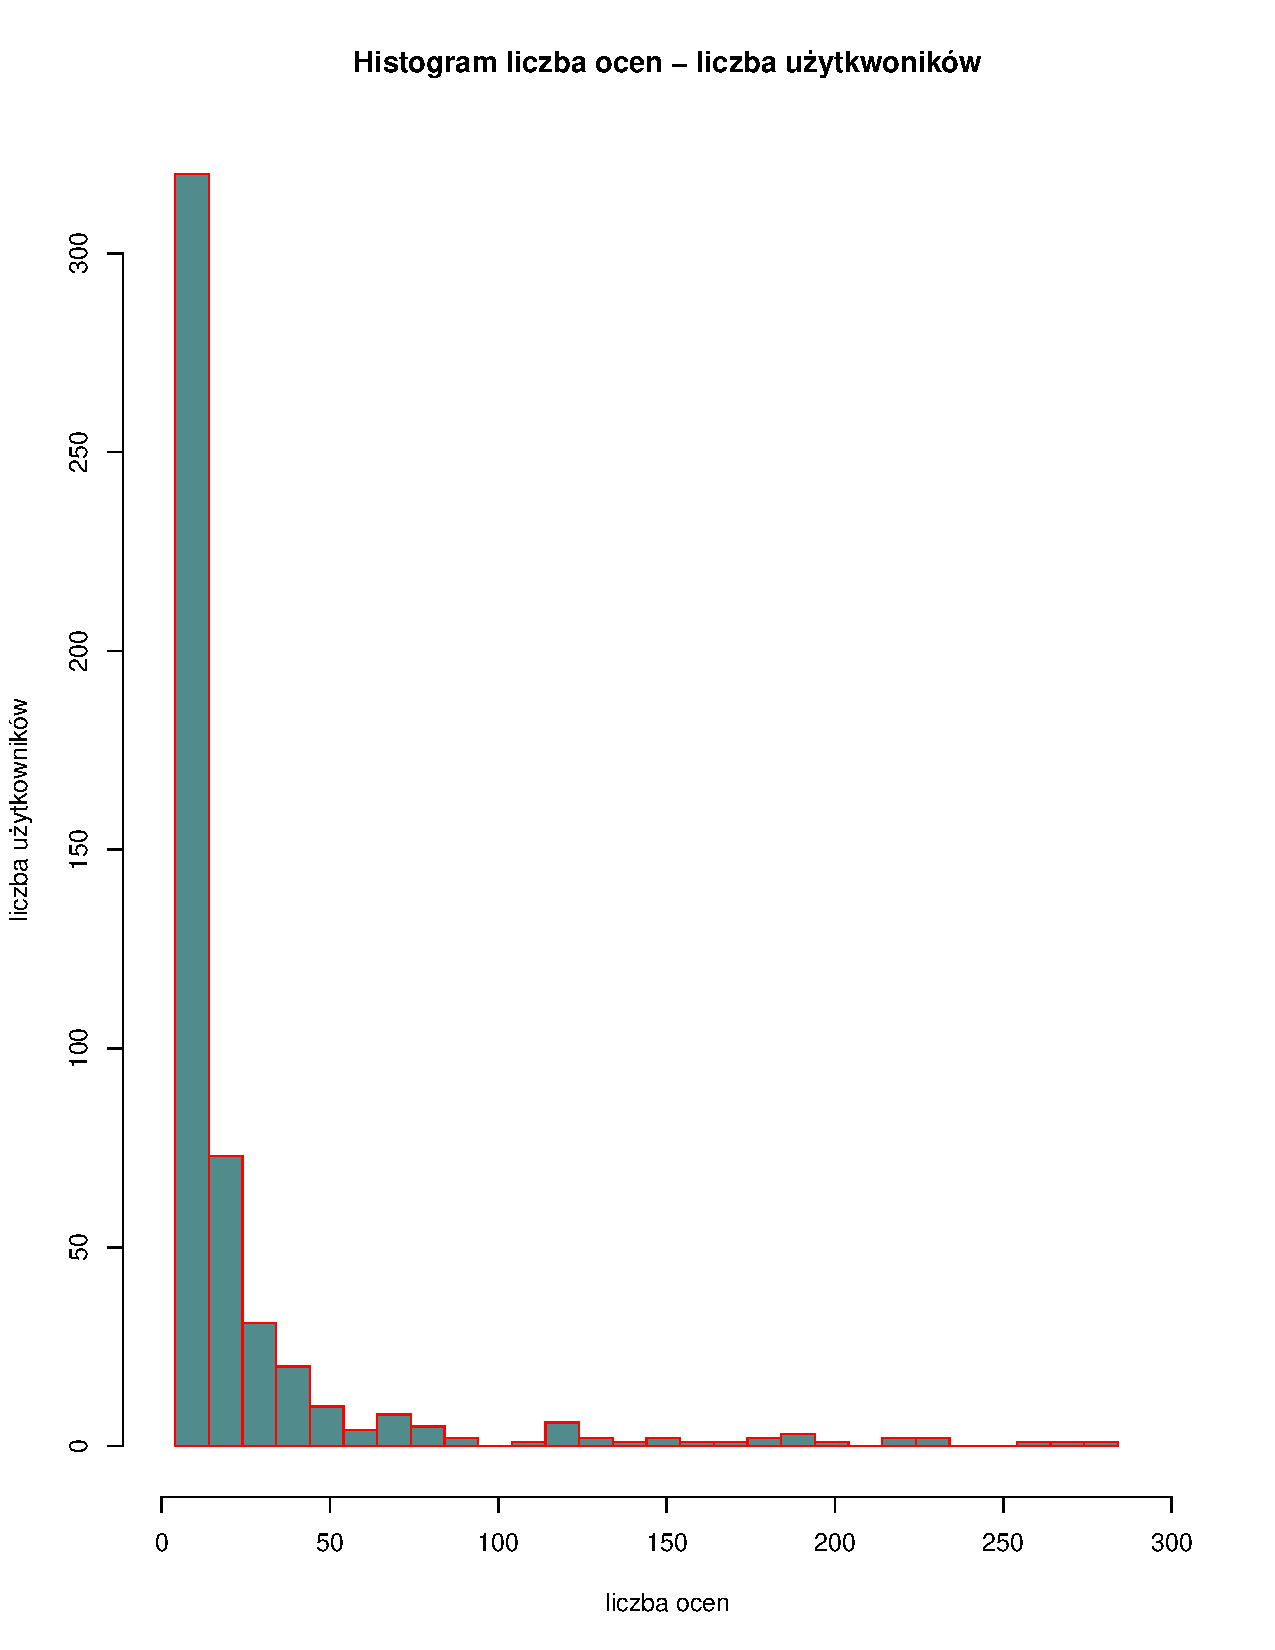
\includegraphics[scale=0.4]{ocenyUzytkownicy.pdf}
\caption[]{Histogram liczba ocen -- liczba użytkowników}
\end{figure}

\subsection{Optymalizacja algorytmu User Based Collaborative Filtering}
\subsubsection{Testy rodzaju normalizacji danych dla UBCF}
\subsubsection{Testy metryk podobieństwa dla UBCF}
\subsubsection{Testy dla różnej ilości najbliższych sąsiadów}
\subsection{Optymalizacja algorytmu Funk SVD}
\subsubsection{Testy rodzaju normalizacji danych dla SVDF}
\subsubsection{Testy dla różnych ilości składowych utajonych SVDF}
\subsubsection{Testy dla różnych współczynników szybkości uczenia SVDF}
\subsection{Porównanie najlepszych modeli}

Wykonano test t -- Studenta dla dwóch populacji:
$$\begin{cases} H_0: \mu_{UBCF} - \mu_{SVDF} = 0\\ 
H_1: \mu_{UBCF} - \mu_{SVDF} \neq 0
\end{cases}$$
gdzie $\mu_{UBCF}, \mu_{SVDF}$ oznaczają średnie arytmetyczne RMSE/MAE z pięciu prób dla najlepszych modeli. W efekcie otrzymano
\begin{itemize}
\item dla RMSE: p--value = 0.5464
\item dla MAE: p--value = 0.4937
\end{itemize}
W obu przypadkach z racji na duże wartości p--value nie mamy podstaw do odrzucenia hipotezy zerowej o równości średnich w obu populacjach.
\subsection{Binaryzacja danych}
\subsection{Proste statystyki}
\section{Uwagi i wnioski}

\newpage
\section{Bibliografia}
\begin{thebibliography}{}
\bibitem{data} \url{https://grouplens.org/datasets/book-crossing/}
\bibitem{recommenderlab1} \url{https://cran.r-project.org/web/packages/recommenderlab/vignettes/recommenderlab.pdf}
\bibitem{recommenderlab2} \url{https://cran.r-project.org/web/packages/recommenderlab/recommenderlab.pdf}
\bibitem{wikiColab} \url{https://en.wikipedia.org/wiki/Collaborative_filtering}
\bibitem{rrecsys} \url{https://cran.r-project.org/web/packages/rrecsys/rrecsys.pdf}
\bibitem{funkSVDWiki} \url{https://en.wikipedia.org/wiki/Matrix\_factorization\_(recommender\_systems)#Funk\_SVD}
\bibitem{funkSVD1} \url{http://nicolas-hug.com/blog/matrix\_facto\_1}
\bibitem{funkSVD2} \url{http://nicolas-hug.com/blog/matrix\_facto\_2}
\bibitem{funkSVD3} \url{http://nicolas-hug.com/blog/matrix\_facto\_3}
\bibitem{slidesSVD} \url{https://www.slideshare.net/DKALab/collaborativefilteringfactorization}
\end{thebibliography}
\end{flushleft}
\end{document}